\begin{figure}[t]
\begin{center}
	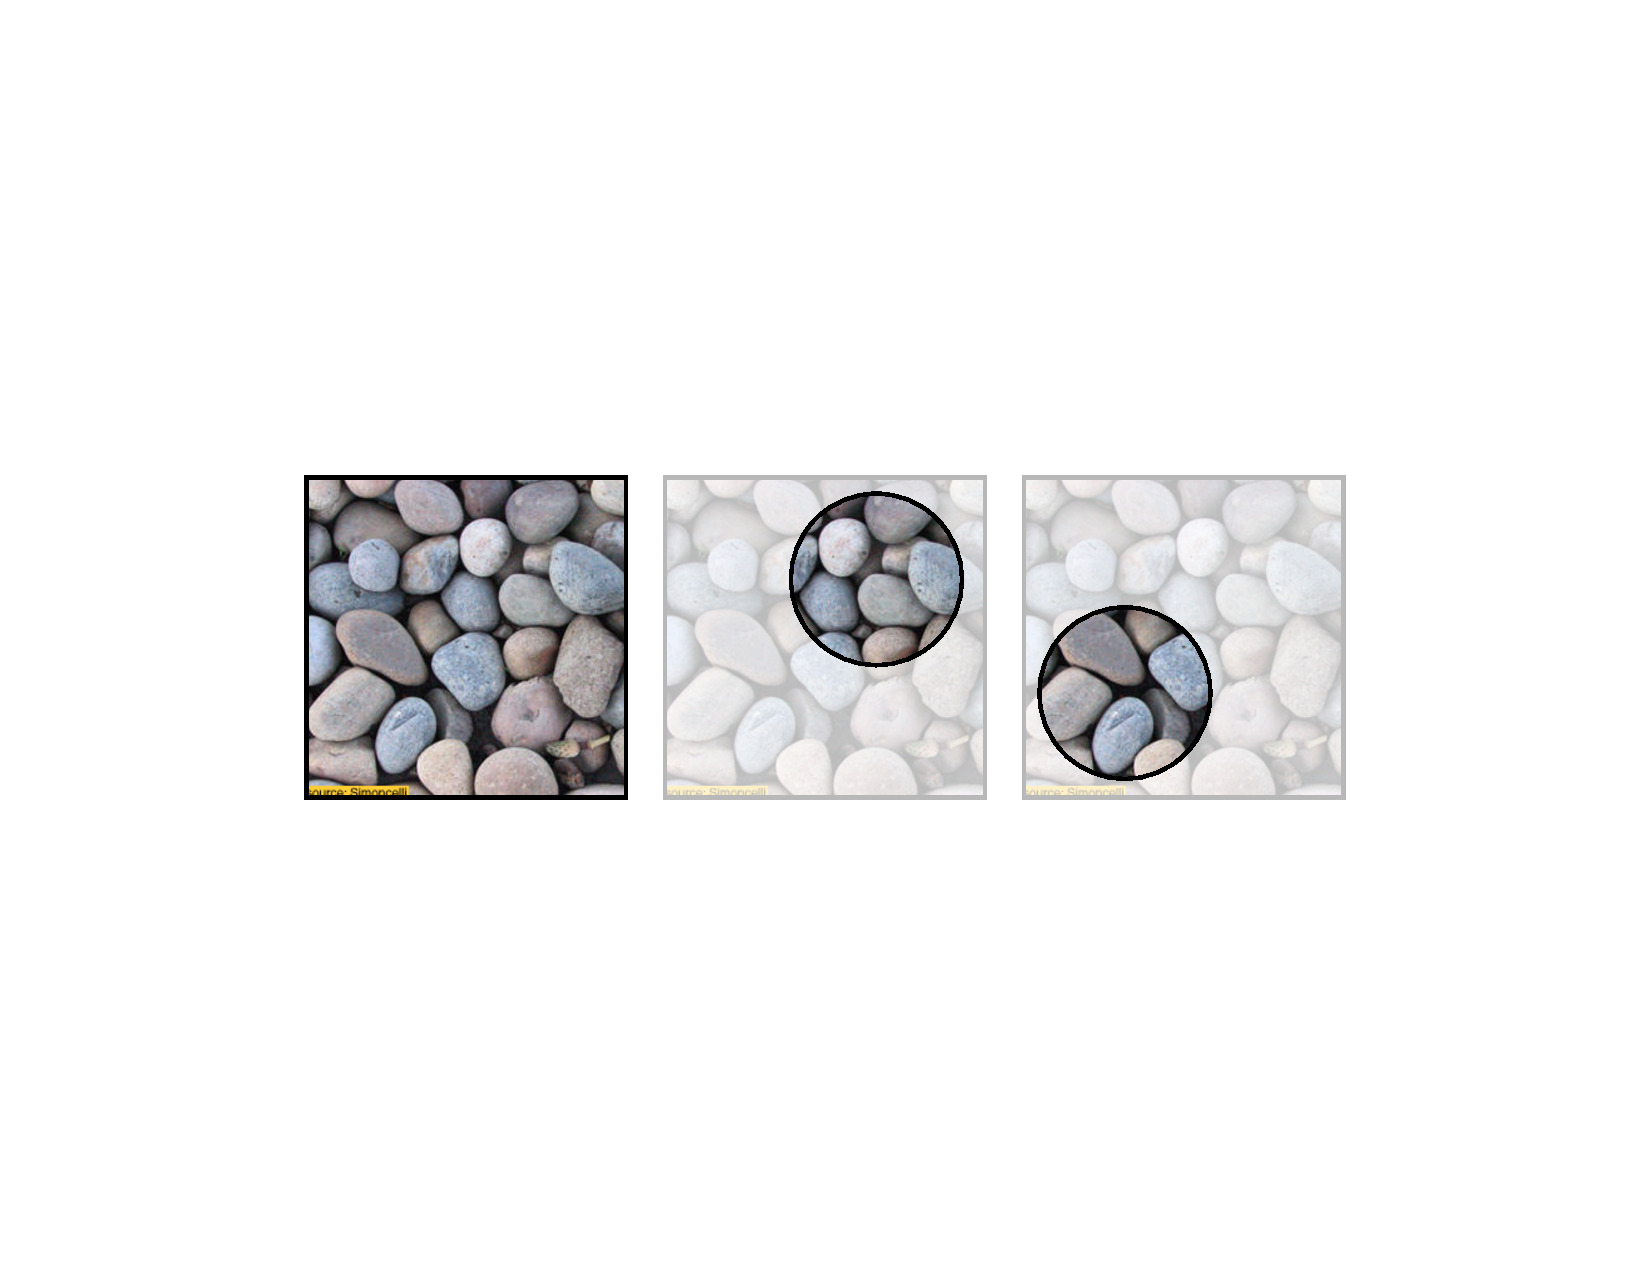
\epsfig{file=texture.pdf, width = 0.8\textwidth}\\
	\caption[A static texture.]{A static texture is a visual pattern that exhibits local spatial variations while maintaining global homogeneity. Observing small apertures across the texture should reveal visual content that looks roughly the same.}
	\vspace{-0.65cm}
	\label{fig:texture}
\end{center}
\end{figure}